% Template for PLoS
% Version 1.0 January 2009
%
% To compile to pdf, run:
% latex plos.template
% bibtex plos.template
% latex plos.template
% latex plos.template
% dvipdf plos.template

\documentclass[10pt]{article}

% amsmath package, useful for mathematical formulas
\usepackage{amsmath}
% amssymb package, useful for mathematical symbols
\usepackage{amssymb}

% graphicx package, useful for including eps and pdf graphics
% include graphics with the command \includegraphics
\usepackage{graphicx}

% cite package, to clean up citations in the main text. Do not remove.
\usepackage{cite}

\usepackage{color} 

% Use doublespacing - comment out for single spacing
%\usepackage{setspace} 
%\doublespacing


% Text layout
\topmargin 0.0cm
\oddsidemargin 0.5cm
\evensidemargin 0.5cm
\textwidth 16cm 
\textheight 21cm

% Bold the 'Figure #' in the caption and separate it with a period
% Captions will be left justified
\usepackage[labelfont=bf,labelsep=period,justification=raggedright]{caption}

% Use the PLoS provided bibtex style
\bibliographystyle{plos2009}

% Remove brackets from numbering in List of References
\makeatletter
\renewcommand{\@biblabel}[1]{\quad#1.}
\makeatother


% Leave date blank
\date{}

\pagestyle{myheadings}
%% ** EDIT HERE **


%% ** EDIT HERE **
%% PLEASE INCLUDE ALL MACROS BELOW

%% END MACROS SECTION

\begin{document}

% Title must be 150 characters or less
\begin{flushleft}
{\Large
\textbf{Diversity Estimation of Metagenomics Samples}
}
% Insert Author names, affiliations and corresponding author email.
%\\
%Qingpeng Zhang$^{1}$, 
%Jason Pell$^{1}$,
%Rosangela Canino-Koning$^{1}$,
%Adina Chuang Howe$^{2,3}$,
%C. Titus Brown$^{1,2\ast}$
%\\
%\bf{1} Computer Science and Engineering, Michigan State University,
%East Lansing, MI, USA
%\\
%\bf{2} Microbiology and Molecular Genetics, Michigan State University,
%East Lansing, MI, USA
%\\
%\bf{3} Plant, Soil, and Microbial Sciences, Michigan State University, 
%East Lansing, MI, USA
%\\
%$\ast$ E-mail: ctb@msu.edu
\end{flushleft}


\section*{Abstract}

Comparison of metagenomics samples
\\
Coverage estimation of metagenomics reads
\\
Diversity evaluation of metagenomics samples

reference-free, assembly-free annotation-free, binning-free


% Please keep the Author Summary between 150 and 200 words
% Use first person. PLoS ONE authors please skip this step. 
% Author Summary not valid for PLoS ONE submissions.   
%\section*{Author Summary}

\section*{Introduction}

% Results and Discussion can be combined.
\section*{Results}

\subsection*{Comparison of metagenomics samples}

\subsubsection*{Theoretical analysis}
\subsubsection*{Synthetic data}
same number of species (100), different composition
\\
same coverage( 20X, 1X)
\\
same error rate ( no error, illumina error profile)
\\
Coverage matters, as expected
\\
after saturation, it can give correct number. if too low coverage, it is not accurate.
But there should be a way to figure out the relationship.
\\
with 1X coverage, 50\% of real coverage.

1x coverage , 63\% of genome is covered

\\next to do:
\\
1. figure out the relationship between coverage and overlap accuracy
\\
2. synthetic data with real bacterial genomes.
\\


two experiments to do 
\\
figure out the ecology of this two levels of diversity difference
\\
3. 

\section*{Discussion}


%\subsection*{TBD}


\section*{Methods}

\subsection*{Code and data set availability}

\subsection*{synthetic data Try 1}
We built 4 series of synthetic data sets:\\
Each series include four sampels with specific composition:\\
SampleA: 100 species with 80 common to B\\
SampleB: 100 species with 80 common to A\\
SampleC: 100 species with 20 common to A/B, and 60 common to D\\
SampleD: 100 species with 20 common to A/B, and 60 common to D\\

4 Series with different coverage and different error rate:\\
1. high coverage(20X) without error\\
2. low coverage(1X) without error\\
3. high coverage(20X) with error, illumina error profile\\
3. low coverage(1X) without error, illumina error profile\\
% @CTB update
%
%The version of khmer used to generate the results below is available
%at http://github.com/ged-lab/khmer.git, tag '2013-khmer-counting'.
%Scripts specific to this paper are available in the paper repository
%at https://github.com/ged-lab/2013-khmer-counting.
%The iPython\cite{4160251} notebook file and data analysis to generate the figures are also
%available in that github repository. 


\subsection*{synthetic data Try 2}

We built 3 series of synthetic data sets:
\\
10 species\\
\\
Sample1A:\\
species IDs:\\
1,2,3,4,5,6,7,8,9,10\\
relative abundance:\\
20:18:16:4:3:2:2:2:2:2\\
\\
Sample1B:\\
species IDs:\\
1,2,3,14,15,16,17,18,19,20\\
relative abundance:\\
20:18:16:4:3:2:2:2:2:2\\
\\
Sample1C:\\
species IDs:\\
21,22,3,4,5,6,7,8,9,10\\
relative abundance:\\
2:2:2:2:2:3:4:16:18:20\\

A and B high overlap on individual level, low overlap on species level\\
A and C high overlap on species level, low overlap on individual level\\
B and C low overlap on species level and low overlap on individual level\\

\\
With error\\
And without error\\
\\
1X  10:9:8:2:1.5:1:1:1:1:1\\
\\
And \\
\\
6X 60:54:48:12:9:6:6:6:6:6\\


Relative abundance matters.\\
We may do diginorm to eliminate the relative abundance firstly then use this method to
 evaluate richness...

%\section*{References}
% The bibtex filename
%\bibliography{khmer-counting}

\section*{Figure Legends}

%\begin{figure}[!ht]
%\begin{center}
%%\includegraphics[width=4in]{figure_name.2.eps}
%\end{center}
%\caption{
%{\bf Bold the first sentence.}  Rest of figure 2  caption.  Caption 
%should be left justified, as specified by the options to the caption 
%package.
%}
%\label{Figure_label}
%\end{figure}


\graphicspath{./figure/}

% @CTB explain why different runs
\begin{figure}[!ht]
\centerline{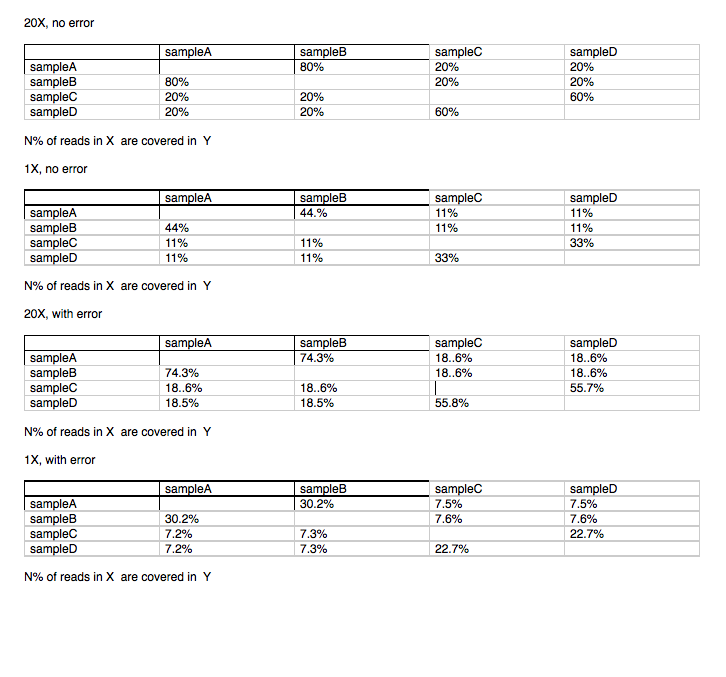
\includegraphics[width=8in]{./figure/figure1}}
\caption{\bf Test 1 \% of reads in sampleX are covered in sampleY }
\label{fig:figure1}
\end{figure}

\begin{figure}[!ht]
\centerline{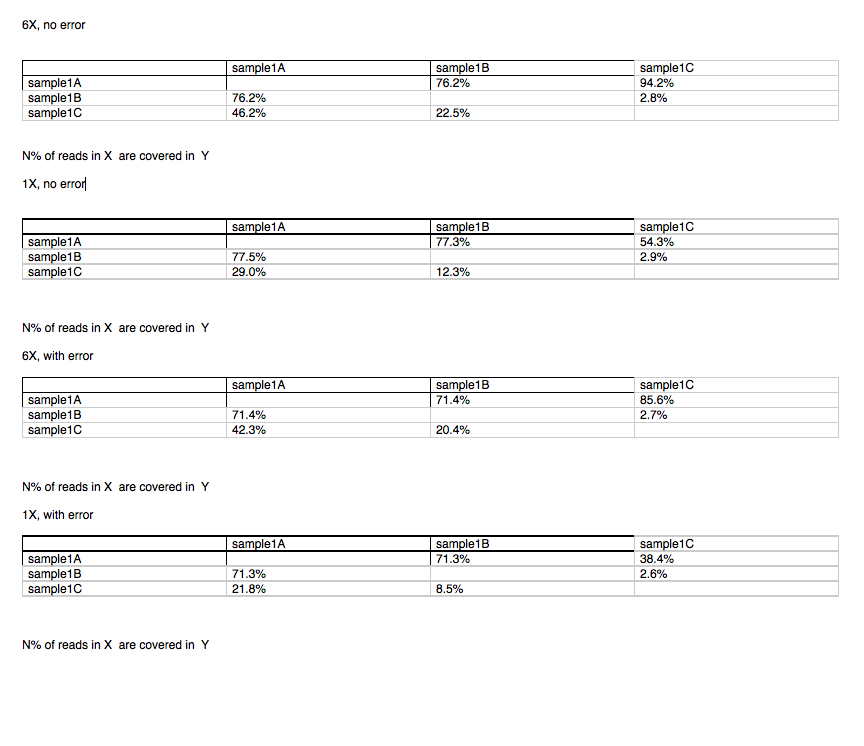
\includegraphics[width=8in]{./figure/figure2}}
\caption{\bf Test 2 \% of reads in sampleX are covered in sampleY }
\label{fig:figure2}
\end{figure}


\section*{Tables}
%\begin{table}[!ht]
%\caption{
%\bf{Table title}}
%\begin{tabular}{|c|c|c|}
%table information
%\end{tabular}
%\begin{flushleft}Table caption
%\end{flushleft}
%\label{tab:label}
% \end{table}

% @CTB fix data set names/descr; caption; reference.
%\begin{table}[!ht]
%\caption{
%\bf{Benchmark soil metagenome data sets for k-mer counting performance, taken from
%\cite{Howe2012}.}}
%\begin{tabular}{ |c | c |c| c|c| }
%Data set & size of file (GB) & number of reads & number of distinct
%k-mers & total number of k-mers \\
%\hline \\
%subset 1        & 1.90 &  9,744,399 &   561,178,082 &   630,207,985 \\
%subset 2        & 2.17 & 19,488,798 & 1,060,354,144 & 1,259,079,821 \\
%subset 3        & 3.14 & 29,233,197 & 1,445,923,389 & 1,771,614,378 \\
%subset 4        & 4.05 & 38,977,596 & 1,770,589,216 & 2,227,756,662 \\
%entire data set & 5.00 & 48,721,995 & 2,121,474,237 & 2,743,130,683 \\
%\end{tabular}
%\begin{flushleft}
%\end{flushleft}
%\label{table:datasets}
%\end{table}
%


\end{document}

